%% IJCAI-format METHOD paper, draft v0.3 (2026-10-18).
%% Changes from v0.2: name fixed to Probe-Gated Critic Transfer; Analysis section with Propositions 1-6 and proofs
%% (Appendix A); explicit assumptions (probe comparability, team separation, drift); local teammate inference wording;
%% 2x2 identifiability x compatibility design; budget-matched random gate; algorithm details; claims hedged.
%% \pilot = single training seed; \tbd = to be filled when runs finish. Earlier drafts: main_v0.1.tex, main_v0.2.tex.
%% Upload the official IJCAI author-kit files (ijcai27.sty or ijcai26.sty, named.bst) next to this file.
\IfFileExists{ijcai27.sty}{\def\ijcaistyle{ijcai27}}{\IfFileExists{ijcai26.sty}{\def\ijcaistyle{ijcai26}}{}}
\ifdefined\ijcaistyle
  \documentclass{article}
\else
  \documentclass[twocolumn,10pt]{article}
\fi
\pdfpagewidth=8.5in
\pdfpageheight=11in
\ifdefined\ijcaistyle
  \usepackage{\ijcaistyle}
\else
  \usepackage[letterpaper,margin=0.75in,columnsep=0.25in]{geometry}
  \usepackage[round]{natbib}
\fi
\usepackage{times}
\usepackage{soul}
\usepackage{url}
\usepackage[utf8]{inputenc}
\usepackage[small]{caption}
\usepackage{graphicx}
\usepackage{amsmath}
\usepackage{amssymb}
\usepackage{amsthm}
\usepackage{booktabs}
\usepackage{xcolor}
\usepackage{algorithm}
\usepackage{algpseudocode}
\urlstyle{same}

\newtheorem{proposition}{Proposition}
\newtheorem{lemma}{Lemma}
\newtheorem{assumption}{Assumption}
\newtheorem{definition}{Definition}
\theoremstyle{remark}
\newtheorem{remark}{Remark}

\newcommand{\todo}[1]{\textcolor{red}{[TODO: #1]}}
\newcommand{\tbd}{\textcolor{red}{TBD}}
\newcommand{\pilot}{\textsuperscript{\textcolor{gray}{$\dagger$}}}
\newcommand{\sg}{\operatorname{sg}}
\newcommand{\JS}{\operatorname{JS}}
\newcommand{\KL}{\operatorname{KL}}
\newcommand{\ours}{PGCT}

\title{Probe-Gated Critic Transfer:\\ Local Teammate Inference for Selective Critic Sharing\\ in Multi-Agent Reinforcement Learning}
\author{Anonymous submission}

\begin{document}
\maketitle

\begin{abstract}
When agents in a shared environment belong to latent teams with different objectives, sharing value estimates
within a team may accelerate learning, but agents rarely know who their teammates are. We study Probe-Gated Critic
Transfer (\ours{}), a decentralised scheme in which neighbouring agents compare their action distributions on a fixed,
pre-agreed bank of probe observations, infer local teammates by thresholding a smoothed Jensen--Shannon divergence, and
distil the critics of inferred teammates on probe inputs. Because behavioural similarity does not in general imply a
shared objective, nor a shared objective a compatible value function, we make the conditions explicit. We show that the
probe divergence is bounded, symmetric and jointly convex, and that its square root is a pseudometric; that thresholding
recovers the local team relation exactly when a separation margin exceeds twice the estimation error, which we bound
through the per-update policy change; that critic distillation is strongly convex in the critic's outputs, so that a wrong
donor biases the receiver by at most a factor $\lambda/(c+\lambda)$ of the value gap; and that teams whose induced
decision problems coincide cannot be separated by any comparison of responses to identical inputs. A team-symmetric
warehouse task instantiates this last case: in a preliminary single-seed run, \ours{} linked agents across teams yet
improved on independent PPO (12\% higher mean and 18\% higher final throughput) and on indiscriminate sharing. A
goal-separated task in which the separation condition can hold is under evaluation \todo{E1-F, seeds, budget-matched gate}.
\end{abstract}

\section{Introduction}
Many multi-agent systems consist of groups that pursue different objectives in a shared space: warehouse robots serving
different clients, vehicles of different fleets, players of different teams. Within a group, sharing what has been
learned---parameters, experience or value estimates---is an effective way to improve sample efficiency in multi-agent
reinforcement learning (MARL) \cite{christianos2020seac,christianos2021seps}; across groups, the same knowledge may
describe a different objective. When group membership is latent, each agent faces three distinct questions:
\emph{(Q1) who is my teammate?} \emph{(Q2) whose critic would help my learning?} and \emph{(Q3) when is the answer to Q1 a
good answer to Q2?}

A tempting decentralised answer to Q1 is to compare behaviour. Two agents that evaluate the same, pre-agreed probe
observations can compare their action distributions without exchanging experience. This is the idea of Probe-Gated
Critic Transfer (\ours{}): neighbours threshold a smoothed Jensen--Shannon (JS) divergence of their probe responses to
infer local teammates, and distil the critics of inferred teammates on probe inputs. The idea rests on two links that do
not hold in general. Behavioural similarity does not imply a shared objective---different objectives can induce the same
action, teammates can play different roles, and untrained policies all look alike---and policies do not identify rewards
\cite{ng2000irl}. A shared objective does not imply compatible value functions---with individual rewards, teammates
compete for the same tasks and differ in competence.

Rather than assume these links, we state when they hold and test them. Our contributions are:
\begin{itemize}
  \item \textbf{Method.} \ours{}, a local, label-free teammate-inference and critic-transfer scheme that exchanges only model
    outputs on a shared probe bank, with all implementation details needed for reproduction (Section~\ref{sec:method}).
  \item \textbf{Analysis.} Properties of the probe divergence; exact local recovery under a separation margin; an estimation
    error bound tied to the per-update policy change; strong convexity of distillation in output space and a bias bound
    for wrong donors; a counterexample showing that policy similarity does not bound value similarity; and a
    non-identifiability result for teams whose induced decision problems coincide (Section~\ref{sec:analysis}).
  \item \textbf{Evaluation design.} Environments placed on two axes---behavioural identifiability of teams and
    within-team critic compatibility---and baselines that separate team selection from the amount of transfer
    (Section~\ref{sec:setup}).
  \item \textbf{Preliminary evidence.} On a team-symmetric task, where our analysis predicts that teams cannot be
    identified, \ours{} indeed did not recover teams but still outperformed independent learning and indiscriminate
    sharing in a single-seed run (Section~\ref{sec:results}). \todo{goal-separated task; seeds; budget-matched gate}
\end{itemize}

\section{Related Work}
\textbf{Selective sharing.} SePS clusters agents before training by an encoding of their transitions and shares parameters
within clusters \cite{christianos2021seps}. MADPS measures distances between agents' policies and adapts parameter
sharing online \cite{hu2024madps}. HetDPS distinguishes several kinds of heterogeneity, including policy and objective
heterogeneity, and shares dynamically according to them \cite{hu2026hetdps}. SEAC shares experience with importance
weighting \cite{christianos2020seac}. Using policy distance to decide whom to share with is therefore not new in itself.
\ours{} differs in the combination of (i) local, online partner selection among current communication neighbours without
a central clustering step, (ii) comparison through a fixed probe bank instead of shared trajectories or parameters, and
(iii) transfer of critic predictions only, with actors trained on private experience. We do not claim novelty for any
single element; we analyse when their combination is justified.

\textbf{Decentralised critics and distillation.} Networked actor-critic methods drive critic parameters to consensus over a
communication graph and come with convergence guarantees for linear function approximation and a network-averaged
objective \cite{zhang2018networked}; these guarantees do not transfer to our individual-reward, nonlinear setting.
\ours{} transfers through distillation on probe inputs \cite{rusu2016policy}.

\textbf{Roles, independent learning and identifiability.} Roles and teams are different latent variables; role-based
methods discover roles from action effects \cite{wang2021rode}. Independent PPO is a strong baseline in cooperative MARL
\cite{schulman2017ppo,dewitt2020ippo}; MAPPO uses a centralised critic \cite{yu2022mappo}. That a policy does not determine
the reward is a classical result in inverse reinforcement learning \cite{ng2000irl}; our non-identifiability result is a
team-level instance. We follow \cite{agarwal2021precipice} for reporting.

\section{Problem Setting}
\label{sec:setting}
We consider a partially observable stochastic game with agents $i\in\{1,\dots,N\}$, observations $o_i^t$, actions
$a_i^t\in\mathcal{A}$ and individual rewards $r_i^t$. Each agent belongs to a latent team $z_i\in\{1,\dots,K\}$ that
determines its objective. Agents know their own objective but not $z_j$ of others. Agents within communication range form
a time-varying neighbourhood $\mathcal{N}_i(t)$. Before training, all agents receive the same probe bank; during training,
neighbours may exchange action probabilities and critic predictions on probe inputs. No observations, experience,
parameters or team labels are exchanged. (Exchanged outputs reveal some information about a policy; we make no privacy
claim.) Each agent learns a recurrent actor $\pi_i$ and critic $V_i$ with PPO.

\begin{definition}[Local team relation]
The local team relation of agent $i$ at time $t$ is $\mathcal{T}_i(t)=\{j\in\mathcal{N}_i(t): z_j=z_i\}$. A method recovers it
if its estimate $\hat{\mathcal{T}}_i(t)$ equals $\mathcal{T}_i(t)$.
\end{definition}

\begin{definition}[Transfer utility]
For a matched pair of updates from the same learning state $\Theta_n$, one using donor $j$ and one independent, the
transfer utility is $U_{i\leftarrow j}=\mathbb{E}[J_i(\Theta^{i\leftarrow j}_{n,+})-J_i(\Theta^{i}_{n,+})]$, where $J_i$ is
agent $i$'s evaluation return \cite{agarwal2021precipice}. Q1 asks for $\mathcal{T}_i$; Q2 asks for donors with
$U_{i\leftarrow j}>0$.
\end{definition}

\section{Probe-Gated Critic Transfer}
\label{sec:method}
\textbf{Probe bank.} All agents hold the same bank $\mathcal{Q}=\{q_m\}_{m=1}^{M}$ of single-step observations, generated by a
deterministic rule from the environment layout before training. A probe is evaluated with zero recurrent state and without
action masking, so a query is one forward pass and leaves training trajectories unchanged.

\begin{assumption}[Probe comparability]
\label{as:comparability}
Every probe $q_m$ is a valid observation for every agent, and it encodes the situation relative to the observing agent's
own objective in the same way for all agents.
\end{assumption}
With team-relative observation channels, the same tensor means ``my requested shelf'' or ``my goal'' to every agent;
probes that would show another team's goal violate the assumption and are excluded by construction (Section~\ref{sec:setup}).

\textbf{Probe divergence.} Let $p_i^m=\pi_i(\cdot\mid q_m,h=0)$. Every $P$ updates, neighbours exchange $\{p_i^m\}_m$ and compute
\begin{equation}
  D_{ij}=\frac{1}{M}\sum_{m=1}^{M}\JS(p_i^m,p_j^m),\quad
  \JS(p,q)=\tfrac12\KL(p\Vert\tfrac{p+q}{2})+\tfrac12\KL(q\Vert\tfrac{p+q}{2}),
  \label{eq:div}
\end{equation}
with natural logarithms, so $D_{ij}\in[0,\ln 2]$ is measured in nats. $D_{ij}$ is the JS \emph{divergence}; its square root
is the JS \emph{distance}.

\textbf{Smoothing and gate.} The first measurement initialises $\bar D_{ij}\gets D_{ij}$; later measurements update
$\bar D_{ij}\gets(1-\beta)\bar D_{ij}+\beta D_{ij}$, only while $i$ and $j$ are neighbours. When they leave each other's
range, $\bar D_{ij}$ and the measurement count $n_{ij}$ are kept but no transfer takes place. After a warm-up of $U_0$ updates,
agent $i$ infers
\begin{equation}
  \hat{\mathcal{T}}_i(t)=\{j\in\mathcal{N}_i(t): n_{ij}\ge n_{\min},\ \bar D_{ij}<\tau\}.
\end{equation}

\textbf{Within-team critic distillation.} With $\alpha_{ij}=1/|\hat{\mathcal{T}}_i(t)|$ for $j\in\hat{\mathcal{T}}_i(t)$ (no peer term if the
set is empty), agent $i$ minimises
\begin{equation}
  \mathcal{L}_i=\mathcal{L}^{\mathrm{PPO}}_i+\lambda\sum_{j\in\hat{\mathcal{T}}_i(t)}\alpha_{ij}\,
  \frac{1}{M_{\mathrm{d}}}\sum_{m=1}^{M_{\mathrm{d}}}\big(V_i(q^{\mathrm{d}}_m)-\sg[V_j(q^{\mathrm{d}}_m)]\big)^2,
  \label{eq:loss}
\end{equation}
where $\mathcal{L}^{\mathrm{PPO}}_i$ is the PPO loss to be minimised (negative clipped surrogate, $c$ times the value loss,
minus an entropy bonus), $\sg$ is the stop-gradient, and donor values are fixed at the start of the update. Both directions
of a pair may be active in the same update; each receiver uses the other's pre-update values. The basic variant distils on
the probe bank itself; \ours{}-v2 uses a separate distillation bank covering all task phases while the inference bank
contains only team-discriminative states.

\textbf{Cost.} A probe round costs $M$ forward passes per agent and exchanges $M|\mathcal{A}|$ probabilities per pair; an active
transfer adds $M_{\mathrm{d}}$ values. With $M=48$, $|\mathcal{A}|=5$, $P=5$ and rollouts of 1{,}024 steps, this is 240 numbers per pair
every 5{,}120 environment steps.

\begin{algorithm}[t]
\caption{\ours{} for agent $i$}
\label{alg:pgct}
\begin{algorithmic}[1]
\State Initialise $\pi_i,V_i$; $\bar D_{ij}\gets$ undefined, $n_{ij}\gets 0$ for all $j$
\For{update $u=1,2,\dots$}
  \State Collect a rollout with $\pi_i$; compute PPO targets from own rewards
  \If{$u\bmod P=0$}
    \For{$j\in\mathcal{N}_i(t)$}
      \State Exchange $\{p^m\}$ on $\mathcal{Q}$; compute $D_{ij}$ (Eq.~\ref{eq:div})
      \State $\bar D_{ij}\gets D_{ij}$ if $n_{ij}=0$ else $(1-\beta)\bar D_{ij}+\beta D_{ij}$; $n_{ij}\gets n_{ij}+1$
    \EndFor
  \EndIf
  \State $\hat{\mathcal{T}}_i\gets\{j\in\mathcal{N}_i(t):n_{ij}\ge n_{\min},\bar D_{ij}<\tau\}$ if $u>U_0$, else $\emptyset$
  \State Receive pre-update $V_j(q^{\mathrm{d}}_m)$ from $j\in\hat{\mathcal{T}}_i$
  \State Update $\pi_i,V_i$ on $\mathcal{L}_i$ (Eq.~\ref{eq:loss}); peer term omitted if $\hat{\mathcal{T}}_i=\emptyset$
\EndFor
\end{algorithmic}
\end{algorithm}

\section{Analysis}
\label{sec:analysis}
Proofs are in Appendix~A. Throughout, $\Delta(\mathcal{A})$ is the probability simplex over actions.

\textbf{The probe divergence.} The JS divergence is used only as a statistic for gating; no gradient flows through it.
Its properties in distribution space are what matter.
\begin{proposition}[Properties]
\label{prop:properties}
(a) $0\le D_{ij}\le\ln 2$, $D_{ij}=D_{ji}$, and $D_{ij}=0$ iff $p_i^m=p_j^m$ for all $m$.
(b) $D_{ij}$ is jointly convex in $(\{p_i^m\}_m,\{p_j^m\}_m)$.
(c) $d_{ij}=\sqrt{D_{ij}}$ is a pseudometric on policies; in particular $d_{ik}\le d_{ij}+d_{jk}$.
\end{proposition}
\begin{remark}
The nonconvexity of $D_{ij}$ in network parameters does not affect optimisation, because $D_{ij}$ is never minimised. The
instability that the gate can cause is of a different kind: a hard threshold makes the set of donors a discontinuous function
of $\bar D_{ij}$, so estimates near $\tau$ can flip the gate between consecutive updates. Propositions~\ref{prop:recovery} and
\ref{prop:tracking} quantify when this cannot change the inferred relation. Part (c) gives approximate transitivity: if $i$ is
close to $j$ and $j$ to $k$, then $i$ is close to $k$.
\end{remark}

\textbf{When does thresholding recover teams?}
\begin{assumption}[Separation]
\label{as:separation}
At update $n$, $\delta_{\mathrm{in}}(n)=\max_{z_i=z_j}D_{ij}(n)$ and $\delta_{\mathrm{out}}(n)=\min_{z_i\ne z_j}D_{ij}(n)$ over current
neighbour pairs satisfy $\Delta(n)=\delta_{\mathrm{out}}(n)-\delta_{\mathrm{in}}(n)>0$.
\end{assumption}
\begin{proposition}[Exact local recovery]
\label{prop:recovery}
Under Assumption~\ref{as:separation}, if $|\bar D_{ij}(n)-D_{ij}(n)|\le\epsilon$ for all neighbour pairs, $2\epsilon<\Delta(n)$,
$\tau\in(\delta_{\mathrm{in}}+\epsilon,\delta_{\mathrm{out}}-\epsilon)$, and warm-up and minimum counts are met, then
$\hat{\mathcal{T}}_i(n)=\mathcal{T}_i(n)$ for every $i$. In particular the inferred relation is symmetric and no wrong donor
is used.
\end{proposition}
The statement is elementary; its value is that it names the two quantities to measure, the margin $\Delta$ and the error
$\epsilon$. Probe responses are deterministic, so $\epsilon$ does not come from sampling noise but from the policies changing
between measurements while the average lags behind.
\begin{lemma}[Drift]
\label{lem:drift}
If between two consecutive measurements every probe response of $i$ and of $j$ changes by at most $\kappa$ in symmetrised KL,
$\KL(p\Vert p')+\KL(p'\Vert p)\le\kappa$, then $|d_{ij}'-d_{ij}|\le\sqrt{\kappa}$ and $|D_{ij}'-D_{ij}|\le2\sqrt{\kappa\ln 2}$.
\end{lemma}
\begin{proposition}[Tracking error]
\label{prop:tracking}
If $|D_{ij}(n)-D_{ij}(n-1)|\le\rho$ for every measurement of the pair, the smoothed estimate initialised with the first
measurement satisfies $|\bar D_{ij}(n)-D_{ij}(n)|\le\frac{1-\beta}{\beta}\rho$. Hence Proposition~\ref{prop:recovery} applies
whenever $2\frac{1-\beta}{\beta}\rho<\Delta(n)$.
\end{proposition}
PPO's clipped objective keeps the average per-update KL on visited states small, which motivates a small $\kappa$; it does not
bound the KL on probe inputs, so Lemma~\ref{lem:drift} is a sufficient condition and we measure $\rho$ directly
\todo{empirical $\rho$ and $\Delta$ from checkpoints}. With $\beta=0.35$ the factor $(1-\beta)/\beta$ is $1.86$; a larger $\beta$
tracks faster but averages less, and hysteresis (two thresholds) is a standard remedy for gate flicker.

\textbf{What does a wrong donor cost?} We idealise the critic at a single probe input $q$ as a free output $v$ with local
regression target $y$ (e.g.\ the receiver's own return estimate) and donor values $v_j$.
\begin{proposition}[Distillation in output space]
\label{prop:bias}
$f(v)=c(v-y)^2+\lambda\sum_j\alpha_{ij}(v-v_j)^2$ with $\sum_j\alpha_{ij}=1$ is $2(c+\lambda)$-strongly convex, with minimiser
$v^\star=\frac{cy+\lambda\sum_j\alpha_{ij}v_j}{c+\lambda}$. If donors in $\hat{\mathcal{T}}_i$ satisfy $|v_j-y|\le\eta$ when
$z_j=z_i$ and $|v_j-y|\le\Gamma$ otherwise, and wrong donors carry mass $a_{\mathrm{w}}$, then
$|v^\star-y|\le\frac{\lambda}{c+\lambda}\big((1-a_{\mathrm{w}})\eta+a_{\mathrm{w}}\Gamma\big)$.
\end{proposition}
With the value-loss coefficient $c=0.5$ and $\lambda=0.01$, the factor $\lambda/(c+\lambda)$ is about $0.02$. In this idealisation
distillation shrinks the critic towards donors by a convex combination; under Proposition~\ref{prop:recovery}, $a_{\mathrm{w}}=0$. The
idealisation ignores that a network shares parameters across inputs and that $c$ weighs rollout states rather than probes; at the
level of parameters, the peer term can conflict with the value loss when
$\langle\nabla\mathcal{L}^V_i,\nabla\mathcal{L}^D_{i\leftarrow j}\rangle<0$, which we propose to monitor as a diagnostic
\todo{gradient-alignment measurement}.

\textbf{When is a team relation a good proxy for compatibility?}
\begin{proposition}[Policy similarity does not bound value similarity]
\label{prop:counter}
There are two agents with $D_{ij}=0$ on every probe and $|V_i-V_j|=1/(1-\gamma)$.
\end{proposition}
The counterexample makes explicit that Q2 is not answered by Q1 alone; compatibility must be measured.

\textbf{When are teams identifiable at all?} Hold the other agents' policies fixed. Agent $i$ then faces a single-agent
decision problem on its own observations. We say that the problems of agents $i$ and $j$ \emph{coincide} if, for every memoryless
observation-to-action map $\mu$, the law of the observation--reward sequence that $i$ experiences when acting by $\mu$ equals the
one that $j$ experiences when acting by $\mu$.
\begin{proposition}[Non-identifiability under team-invariant decision problems]
\label{prop:nonid}
If the decision problems induced on agents of different teams coincide as functions of their observations, then, within
memoryless policies, every observation-to-action map that is optimal for one team is optimal for the other. If the optimal map is unique, any
objective-optimal policies satisfy $D_{ij}=0$ for all pairs, so $\Delta=0$ and no threshold separates teams. Differences in
probe responses then reflect non-objective factors such as roles or learning progress.
\end{proposition}
Team-relative observations together with mirror-symmetric tasks produce exactly this case. If instead the observation contains
quantities whose meaning does not change with the team (for example the agent's absolute position) while the teams' goals
differ, the induced decision problems differ and Proposition~\ref{prop:nonid} does not apply.

\section{Experimental Design}
\label{sec:setup}
\textbf{Environments on two axes.} We use a two-team variant of the multi-robot warehouse \cite{papoudakis2021benchmarking}
on an $11\times10$ map with four agents (agents 1, 3 in team red; 2, 4 in team blue). Each team always has two requested
shelves and its own goal; half of each team's shelves lie in the other team's half. Observations are egocentric $11\times11$
semantic grids with team-relative channels plus ego features including the absolute position. Rewards are individual.

\begin{table}[t]
\centering
\small
\resizebox{\columnwidth}{!}{%
\begin{tabular}{lcc}
\toprule
 & Within-team critics compatible & Not compatible \\
\midrule
Teams identifiable by behaviour & E1-F + team reward (planned) & E1-F (individual reward)? \\
Not identifiable & -- & E1 (measured) \\
\bottomrule
\end{tabular}}
\caption{Environments placed on the two axes of the analysis. E1: identifiability ruled out by Proposition~\ref{prop:nonid};
within-team compatibility measured to be lower than across teams. E1-F: identifiability expected; compatibility to be measured.
\todo{place E1-F after measurement}}
\label{tab:axes}
\end{table}

\begin{itemize}
  \item \textbf{E1 (team-symmetric).} Goals adjacent at the bottom centre. With team-relative channels both teams face the
    same decision problem, so Proposition~\ref{prop:nonid} applies.
  \item \textbf{E1-F (goal-separated).} Goals at opposite bottom corners. A loaded agent must head to its own corner; since the
    observation contains the absolute position, the decision problems differ and teams can be identifiable.
  \item \textbf{E1-F with team reward} (planned): delivery and return rewards are shared within the team, so teammates share a
    value target.
\end{itemize}

\textbf{Probe banks.} The canonical bank has 48 states covering pickup, delivery and return. The v2 inference bank has 48 states
in which an agent carries a requested shelf and \emph{no goal of any team} is visible, so the same input is valid for every agent
(Assumption~\ref{as:comparability}) and the action depends on where the agent's own team delivers; the v2 distillation bank has 64
states balanced over task phases. All probes are realised in the training environment and validated.

\textbf{Methods.} IPPO (no transfer), All-peer (every neighbour), Oracle-team (ground-truth teammates among neighbours; a privileged
reference, not an upper bound), \ours{} and \ours{}-v2. To separate \emph{whom} to share with from \emph{how much}, we add
Random-gated transfer, which draws donors uniformly among neighbours at the realised per-update donor count of \ours{}, and a
budget-matched Oracle \todo{implement and run}. All methods start from bit-identical weights for a given seed and differ only in
the donor set. \ours{} uses $P=5$, $\beta=0.35$, $\tau=0.12$ nats, $U_0=100$, $n_{\min}=8$, $\lambda=0.01$, $c=0.5$
(Appendix~B).

\textbf{Measures.} \emph{Learning}: delivery onset (first step at which the 3-point moving average reaches one delivery per
episode), mean deliveries per episode over training, final deliveries (last five evaluations), number of agents that learned.
\emph{Inference}: precision, recall and F1 of $\hat{\mathcal{T}}_i$ against $\mathcal{T}_i$ over realised updates; same-team AUROC
of $D_{ij}$ on checkpoints; the empirical margin $\Delta$ and drift $\rho$. \emph{Compatibility}: reduction of the receiver's value
error when its critic is blended with a teammate's vs.\ a non-teammate's. \emph{Transfer}: realised donors per update and the
share of within-team arcs. Evaluation uses 20 episodes of 500 steps every 51{,}200 steps with a deterministic masked policy.

\section{Results}
\label{sec:results}
\textbf{Status.} E1 has one training seed, stopped at 6.5M steps (statistics on the common horizon of 6.4M; marked \pilot). E1-F
runs for all methods except the random gate are in progress. \todo{seeds 2--$n$; E1-F; random gate}

\begin{table}[t]
\centering
\small
\resizebox{\columnwidth}{!}{%
\begin{tabular}{lcccccc}
\toprule
Method & Labels & Onset$\downarrow$ & Mean$\uparrow$ & Final$\uparrow$ & Learned & Mean ($n$ seeds) \\
\midrule
IPPO & -- & 2.05M & 10.4 & 23.2 $\pm$ 1.1 & 2/4 & \tbd \\
All-peer & -- & 3.99M & 3.7 & 19.4 $\pm$ 1.6 & 4/4 & \tbd \\
Random-gated & -- & \tbd & \tbd & \tbd & \tbd & \tbd \\
\textbf{\ours{}} & -- & 1.79M & 11.7 & 27.3 $\pm$ 1.4 & 3/4 & \tbd \\
\midrule
Oracle-team & team & 1.64M & 13.2 & 32.2 $\pm$ 1.7 & 3/4 & \tbd \\
\bottomrule
\end{tabular}}
\caption{E1 (team-symmetric), one seed\pilot, common horizon 6.4M steps. Final: mean $\pm$ s.d.\ over the last five evaluations
(not seeds). Learned: agents with at least one delivery per episode at the end.}
\label{tab:e1}
\end{table}

\begin{figure}[t]
\centering
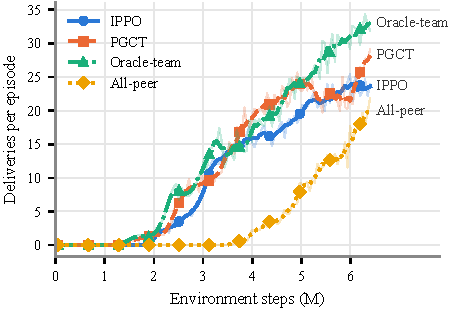
\includegraphics[width=\columnwidth]{figures/fig1_learning_curves.pdf}
\caption{Evaluation deliveries per episode on E1 (one seed\pilot). Thin: raw evaluations; thick: centred 5-point moving average.}
\label{fig:curves}
\end{figure}

\textbf{Learning on E1.} \ours{} improved on independent learning on every measure (Table~\ref{tab:e1},
Figure~\ref{fig:curves}):\pilot{} one delivery per episode 0.26M steps earlier, 12\% higher mean and 18\% higher final throughput, and
the first to reach 20 deliveries per episode (4.15M steps vs.\ 4.66M for Oracle-team and 5.07M for IPPO). All-peer delayed the onset
by about two million steps. Per agent (Appendix~D), IPPO trained only one deliverer per team; \ours{} and Oracle-team trained a third
agent and All-peer all four, albeit late. We hypothesise that distilling a competent peer's critic gives an agent that receives
little reward of its own a learning signal; an intervention that blocks transfer to that agent is needed to test this
\todo{intervention}.

\begin{figure*}[t]
\centering
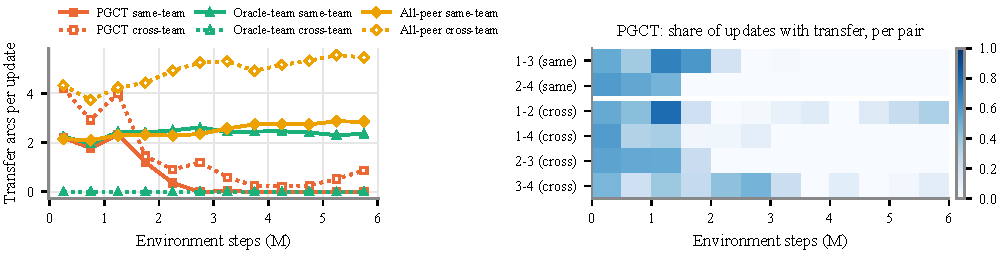
\includegraphics[width=\textwidth]{figures/fig3_critic_transfer.pdf}
\caption{Realised critic transfer on E1 (one seed\pilot). Left: directed transfer arcs per update within (solid) and across (dotted)
teams, 0.5M-step bins. Right: for \ours{}, share of updates in which each pair exchanged critic information.}
\label{fig:transfer}
\end{figure*}

\textbf{Inference on E1 matches the analysis.} Proposition~\ref{prop:nonid} predicts that teams are not identifiable on E1. Indeed,
from 2.5M steps on, the probe divergence between teammates exceeded that between non-teammates at almost every checkpoint and for
every method (Appendix~D), i.e.\ the empirical margin was negative, and the same held on frozen models for five probe subsets
including the v2 inference bank. Accordingly, \ours{} did not recover teams: after 4M steps, 95\% of its transfer arcs connected
agents of different teams (0.03 vs.\ 0.63 arcs per update; Figure~\ref{fig:transfer}), namely agents with the same role (staying in
the own half vs.\ fetching shelves from the other half). Three explanations of the performance gain are therefore possible:
transfer between teammates (H1), selective transfer between behaviourally similar agents regardless of team (H2), or simply less
transfer than All-peer (H3; \ours{} transferred on 29--37\% of updates after 2M steps, All-peer on almost all). The E1 data rule
out H1 as the cause; the budget-matched random gate will separate H2 from H3 \todo{random gate}. Consistently with H2, in an
independent frozen evaluation, blending a receiver's critic with a non-teammate's reduced its value error more than blending with a
teammate's (same-team AUROC 0.25--0.33), so cross-team links were not harmful here.

\textbf{Goal-separated teams (E1-F).} \todo{Fill: (1) Oracle-team vs.\ All-peer; (2) within- vs.\ cross-team compatibility; (3)
precision/recall of $\hat{\mathcal{T}}_i$, AUROC, $\Delta$ and $\rho$ for \ours{} and \ours{}-v2; (4) learning vs.\ IPPO, All-peer,
Random-gated, Oracle-team.}

\begin{table}[t]
\centering
\small
\resizebox{\columnwidth}{!}{%
\begin{tabular}{lcccccc}
\toprule
Method & Onset & Mean & Final & Precision & Recall & $\Delta$ \\
\midrule
IPPO & \tbd & \tbd & \tbd & -- & -- & \tbd \\
All-peer & \tbd & \tbd & \tbd & \tbd & \tbd & \tbd \\
Random-gated & \tbd & \tbd & \tbd & \tbd & \tbd & \tbd \\
\ours{} & \tbd & \tbd & \tbd & \tbd & \tbd & \tbd \\
\ours{}-v2 & \tbd & \tbd & \tbd & \tbd & \tbd & \tbd \\
Oracle-team & \tbd & \tbd & \tbd & 1 & 1 & \tbd \\
\bottomrule
\end{tabular}}
\caption{E1-F (goal-separated). Precision and recall of the inferred local team relation over realised updates; $\Delta$: empirical
separation margin of the probe divergence. \todo{fill when the runs finish}}
\label{tab:e1f}
\end{table}

\section{Discussion and Limitations}
\textbf{What the analysis does and does not give.} Propositions~\ref{prop:recovery}--\ref{prop:bias} turn the informal chain
``similar behaviour $\Rightarrow$ same team $\Rightarrow$ useful critic'' into checkable conditions: a positive margin, a small drift,
and compatible teammates' values. Propositions~\ref{prop:counter} and \ref{prop:nonid} show that the first and second links can
fail, and E1 is an instance of the second failure. We give no convergence guarantee for the coupled learning dynamics.

\textbf{Team discovery or compatibility discovery.} Our target is teammate inference (Q1) because team relations are what a
designer often wants to respect. When teams are not identifiable, or when compatibility does not follow team membership, a gate
that targets transfer utility directly (Q2) is the more general goal; the probe divergence can then be read as a proxy whose
usefulness must be measured, e.g.\ by the rank correlation between $D_{ij}$ and estimated $U_{i\leftarrow j}$.

\textbf{Assumptions and scope.} \ours{} requires a shared probe bank satisfying Assumption~\ref{as:comparability}; our bank is
constructed by a fixed rule from the map layout, and probe sensitivity (number, design, random probes) must be reported
\todo{probe ablation}. Single-step zero-state probes suffice when the observation contains the agent's position, as here; histories
may be needed otherwise. Agents could exchange team identifiers if they had a common vocabulary; teammate inference is relevant when
objectives are private or labels are not shared. We evaluate one environment family with four agents and two teams, and the E1
results come from one seed; re-running the same seed reproduced IPPO exactly but not the sharing variants (Appendix~D).

\section{Conclusion}
We studied Probe-Gated Critic Transfer, which infers local teammates from responses to a shared probe bank and distils their critics.
We made the conditions under which this is justified explicit---separation, bounded drift, compatible values---and showed when they
fail, including a non-identifiability result for teams whose decision problems coincide. On such a team-symmetric task \ours{} did not
recover teams, as predicted, yet improved learning in a preliminary run; whether it recovers teams and helps when the conditions hold
is being evaluated on a goal-separated task.

\ifdefined\ijcaistyle
  \bibliographystyle{named}
\else
  \bibliographystyle{plainnat}
\fi
\bibliography{references}

\clearpage
\appendix
\onecolumn

\section{Proofs}

\textbf{Proposition~\ref{prop:properties}.}
(a) For $m=\frac{p+q}{2}$, $\KL(p\Vert m)=\sum_a p(a)\ln\frac{2p(a)}{p(a)+q(a)}\le\sum_a p(a)\ln 2=\ln 2$, and similarly for $q$; hence
$0\le\JS\le\ln2$. Symmetry is immediate. $\JS(p,q)=0$ iff $\KL(p\Vert m)=\KL(q\Vert m)=0$ iff $p=m=q$. Averaging over probes preserves
all three statements, with equality to zero iff every term is zero.
(b) $\JS(p,q)=\sum_a q(a)\,\phi\!\big(p(a)/q(a)\big)$ with $\phi(t)=\frac{t}{2}\ln\frac{2t}{1+t}+\frac12\ln\frac{2}{1+t}$, which is convex
with $\phi(1)=0$; $\JS$ is therefore an $f$-divergence, and $f$-divergences are jointly convex in their two arguments (perspective of a
convex function). A sum of jointly convex functions of disjoint coordinates is jointly convex.
(c) $\sqrt{\JS}$ is a metric on $\Delta(\mathcal{A})$ \cite{endres2003metric}. For $x_m=\sqrt{\JS(p_i^m,p_k^m)}$,
$y_m=\sqrt{\JS(p_i^m,p_j^m)}$, $w_m=\sqrt{\JS(p_j^m,p_k^m)}$ we have $x_m\le y_m+w_m$, and by Minkowski's inequality
$\big(\frac1M\sum_m x_m^2\big)^{1/2}\le\big(\frac1M\sum_m y_m^2\big)^{1/2}+\big(\frac1M\sum_m w_m^2\big)^{1/2}$, i.e.\
$d_{ik}\le d_{ij}+d_{jk}$. Symmetry and $d_{ii}=0$ follow from (a). It is a pseudometric because policies that agree on $\mathcal{Q}$ have
$d=0$.

\textbf{Proposition~\ref{prop:recovery}.} If $z_i=z_j$, then $\bar D_{ij}\le D_{ij}+\epsilon\le\delta_{\mathrm{in}}+\epsilon<\tau$, so
$j\in\hat{\mathcal{T}}_i$. If $z_i\ne z_j$, then $\bar D_{ij}\ge D_{ij}-\epsilon\ge\delta_{\mathrm{out}}-\epsilon>\tau$, so
$j\notin\hat{\mathcal{T}}_i$. The interval for $\tau$ is non-empty iff $2\epsilon<\Delta$. Symmetry follows because the conditions do not
depend on the order of $i$ and $j$.

\textbf{Lemma~\ref{lem:drift}.} By joint convexity of $\KL$, $\KL(p\Vert\frac{p+p'}{2})\le\frac12\KL(p\Vert p)+\frac12\KL(p\Vert p')=\frac12\KL(p\Vert p')$,
and likewise $\KL(p'\Vert\frac{p+p'}{2})\le\frac12\KL(p'\Vert p)$. Hence $\JS(p,p')\le\frac14(\KL(p\Vert p')+\KL(p'\Vert p))\le\kappa/4$. By the
triangle inequality for $\sqrt{\JS}$ on each probe,
$|\sqrt{\JS(p_i'^m,p_j'^m)}-\sqrt{\JS(p_i^m,p_j^m)}|\le\sqrt{\JS(p_i^m,p_i'^m)}+\sqrt{\JS(p_j^m,p_j'^m)}\le\sqrt{\kappa}$. Minkowski's
inequality over probes gives $|d'_{ij}-d_{ij}|\le\sqrt{\kappa}$, and $|D'-D|=|d'-d|(d'+d)\le\sqrt{\kappa}\cdot2\sqrt{\ln 2}$ by
Proposition~\ref{prop:properties}(a).

\textbf{Proposition~\ref{prop:tracking}.} Let $e_n=\bar D(n)-D(n)$. Then $e_n=(1-\beta)\bar D(n-1)+\beta D(n)-D(n)=(1-\beta)e_{n-1}+(1-\beta)(D(n-1)-D(n))$,
so $|e_n|\le(1-\beta)|e_{n-1}|+(1-\beta)\rho$. With $e_1=0$ (initialisation with the first measurement),
$|e_n|\le(1-\beta)\rho\sum_{k\ge0}(1-\beta)^k=\frac{1-\beta}{\beta}\rho$.

\textbf{Proposition~\ref{prop:bias}.} $f''(v)=2c+2\lambda\sum_j\alpha_{ij}=2(c+\lambda)$, so $f$ is $2(c+\lambda)$-strongly convex and has the
unique stationary point $v^\star$ given. Then $v^\star-y=\frac{\lambda}{c+\lambda}\sum_j\alpha_{ij}(v_j-y)$, and the triangle inequality with the
stated bounds on $|v_j-y|$ gives the result.

\textbf{Proposition~\ref{prop:counter}.} Take a single state, a single action and $\mathcal{Q}=\{q\}$ with both agents' policies the point mass on that
action, so $D_{ij}=0$. Let $r_i\equiv0$ and $r_j\equiv1$; then $V_i=0$ and $V_j=\sum_t\gamma^t=1/(1-\gamma)$.

\textbf{Proposition~\ref{prop:nonid}.} With the other agents fixed, the expected discounted return of a memoryless map $\mu$ for agent $i$ is a
functional of the law of the observation--reward sequence that $i$ experiences under $\mu$. If these laws coincide for agents $i$ and $j$ of
different teams for every $\mu$, then every $\mu$ has the same return for both, so the sets of optimal memoryless maps coincide. If the optimal map $\mu^\star$ is unique, every objective-optimal policy equals $\mu^\star$ on every observation, including every
probe, so $p_i^m=p_j^m$ and $D_{ij}=0$ for all pairs. Then $\delta_{\mathrm{in}}=\delta_{\mathrm{out}}=0$ and $\Delta=0$, and no $\tau$ satisfies
$\delta_{\mathrm{in}}<\tau\le\delta_{\mathrm{out}}$.

\section{Hyper-parameters}
\begin{table}[h]
\centering
\small
\begin{tabular}{ll}
\toprule
Setting & Value \\
\midrule
Map / agents / teams & 11$\times$10 E1 / 4 / 2 \\
Reward & individual \\
Home-zone shelf ratio & 0.5 \\
Requests per team & 2 \\
Sensor / communication range & 5 / 5 \\
Learning rate & 0.0002 \\
Entropy coef. & 0.05 \\
$\gamma$ / GAE $\lambda$ & 0.99 / 0.95 \\
Rollout / BPTT length & 1024 / 64 \\
PPO epochs / minibatches / clip & 4 / 8 / 0.2 \\
Hidden (MLP / GRU) & 128 / 128 \\
Peer-loss coef. $\lambda_{peer}$ & 0.01 \\
Gate: JS threshold / EMA $\beta$ / warm-up & 0.12 / 0.35 / 100 upd. \\
Canonical probes & 48 (fixed, zero hidden, length 1) \\
Evaluation & every 50 updates, 20$\times$500 steps, deterministic \\
\bottomrule
\end{tabular}

\caption{Settings of the from-scratch E1 comparison (identical for all methods except the donor set).}
\end{table}

\section{Realised transfer per window}
\begin{table}[h]
\centering
\small
\begin{tabular}{llccc}
\toprule
Method & Window & Updates w/ transfer & Same-team arcs/upd. & Cross-team arcs/upd. \\
\midrule
PGCT & 0--2.0M & 91\% & 1.86 & 3.09 \\
 & 2--4.0M & 37\% & 0.10 & 0.73 \\
 & 4--6.4M & 29\% & 0.03 & 0.63 \\
\addlinespace
Oracle-team & 0--2.0M & 82\% & 2.26 & 0.00 \\
 & 2--4.0M & 86\% & 2.50 & 0.00 \\
 & 4--6.4M & 85\% & 2.39 & 0.00 \\
\addlinespace
All-peer & 0--2.0M & 99\% & 2.22 & 4.18 \\
 & 2--4.0M & 100\% & 2.49 & 5.10 \\
 & 4--6.4M & 100\% & 2.79 & 5.37 \\
\bottomrule
\end{tabular}

\caption{Realised transfer on E1 per training window (one seed). Arcs are directed receiver--donor links.}
\end{table}

\section{Additional E1 results}
\begin{figure}[h]
\centering
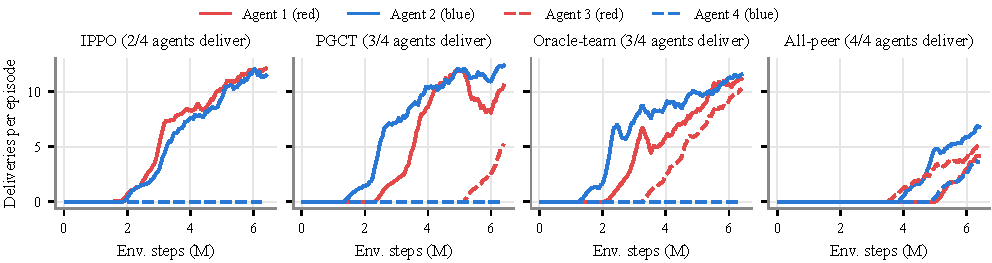
\includegraphics[width=\textwidth]{figures/fig2_per_agent_deliveries.pdf}
\caption{Deliveries per episode of each agent on E1 (5-point moving average; one seed). Red: team red (agents 1, 3); blue: team blue
(agents 2, 4); solid: agents 1--2; dashed: agents 3--4.}
\end{figure}
\begin{figure}[h]
\centering
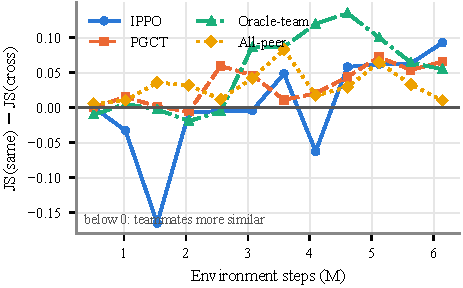
\includegraphics[width=0.6\textwidth]{figures/fig4_probe_js_gap.pdf}
\caption{Probe divergence between teammates minus that between non-teammates on E1 checkpoints (one seed). Above zero: teammates differ
more, i.e.\ the empirical margin is negative.}
\end{figure}
\begin{figure}[h]
\centering
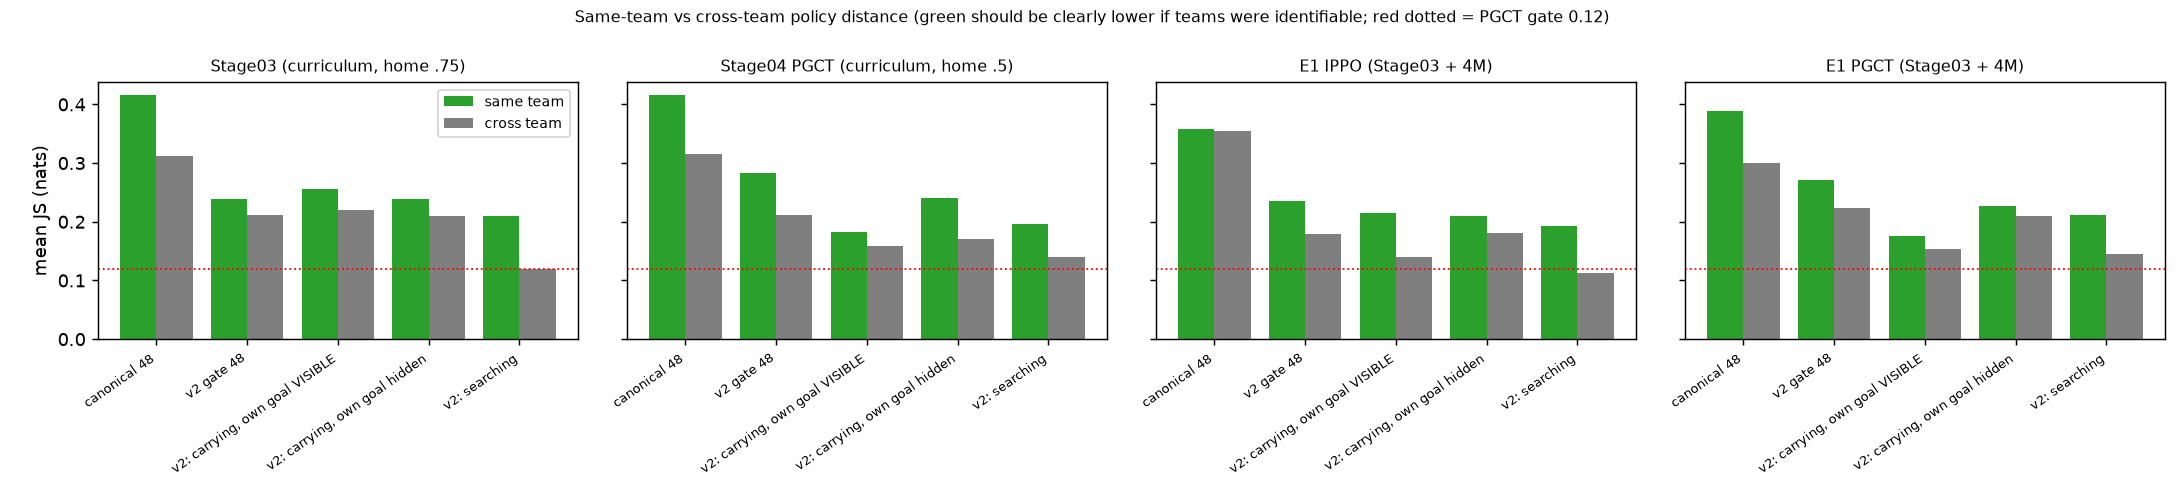
\includegraphics[width=\textwidth]{figures/frozen_probe_same_vs_cross.png}
\caption{Mean probe divergence between teammates (green) and non-teammates (grey) for four frozen E1 models and five probe subsets, including
the v2 inference bank. Teammates are less similar in all 20 combinations. Red dotted line: $\tau=0.12$.}
\end{figure}
\begin{figure}[h]
\centering
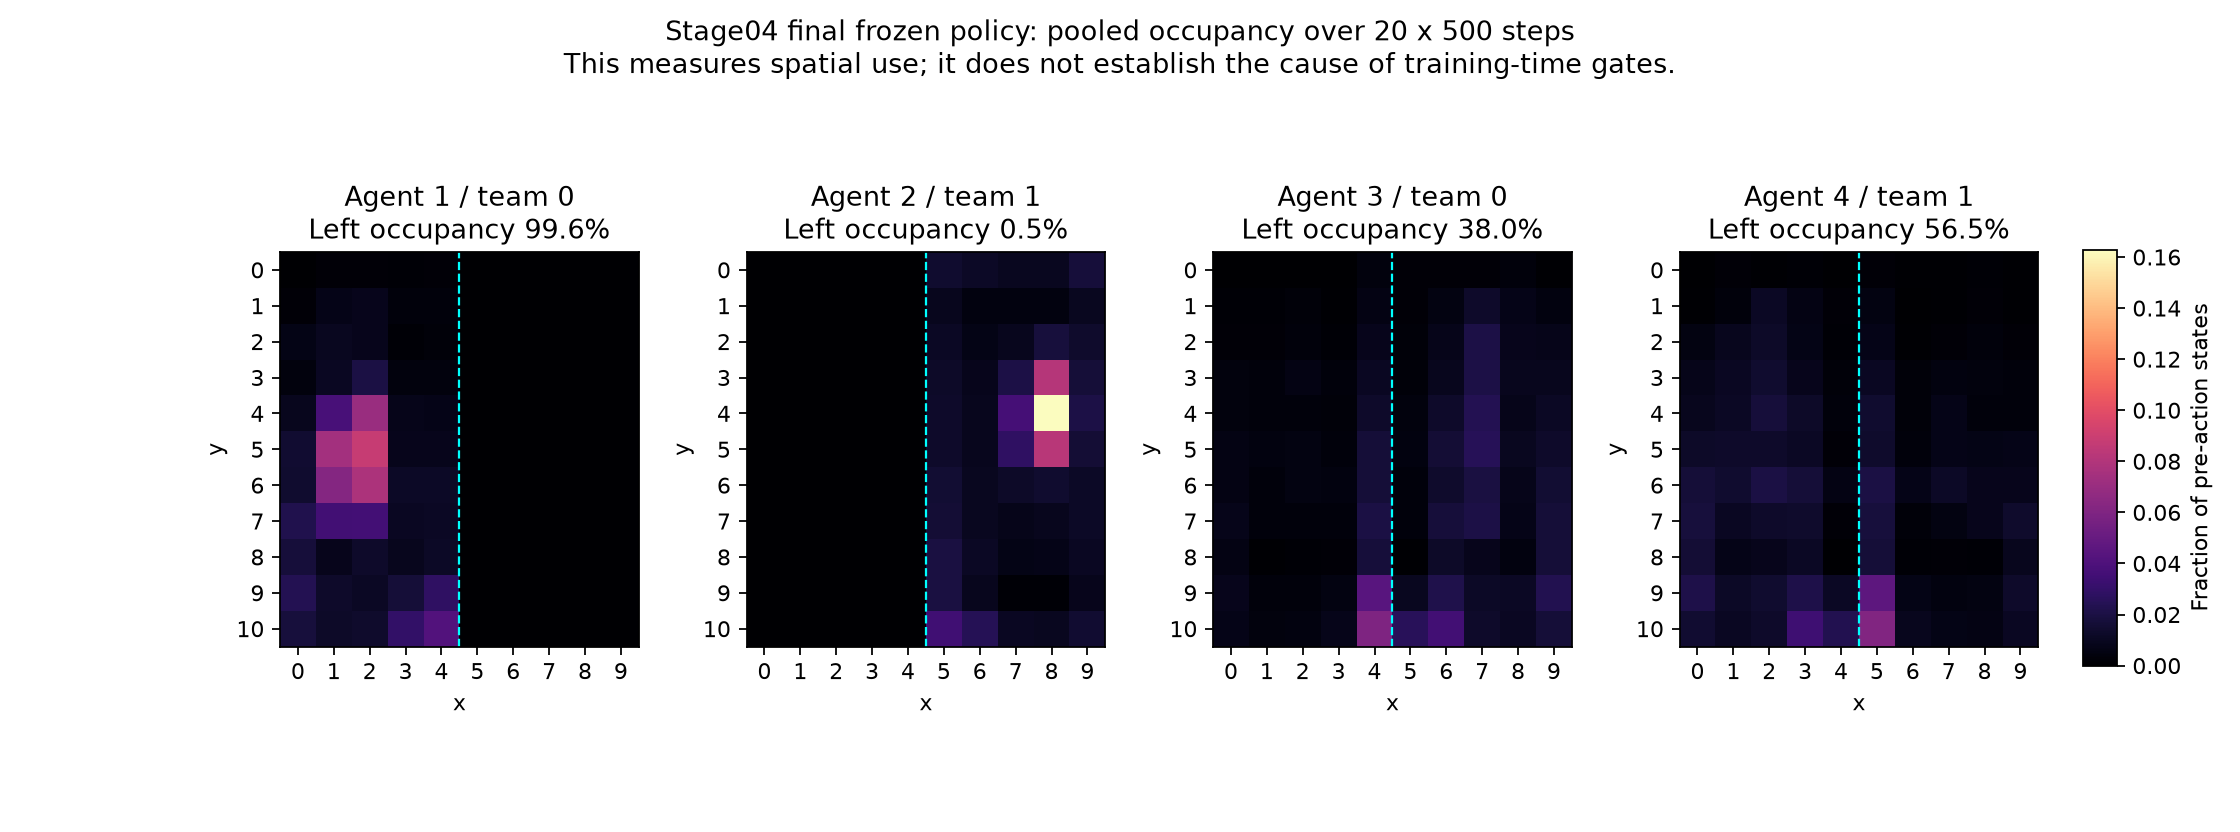
\includegraphics[width=\textwidth]{figures/stage04_occupancy.png}
\caption{Cell occupancy of a frozen curriculum model (50\% of shelves in the other team's half). Agents 1 and 2 stay in their team's half;
agents 3 and 4 fetch shelves from the other half and are the pair the gate linked most often.}
\end{figure}
\begin{figure}[h]
\centering
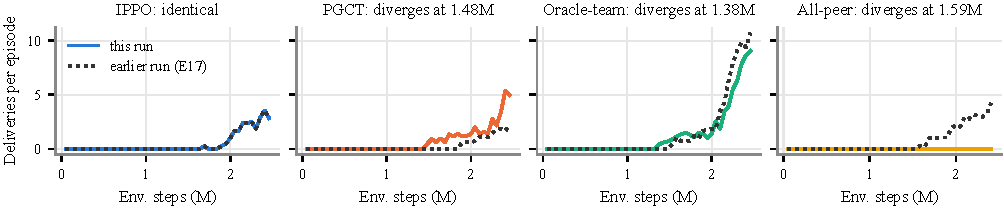
\includegraphics[width=\textwidth]{figures/figA1_reproducibility.pdf}
\caption{Same seed and initial weights, two runs (solid: reported; dotted: earlier interrupted run). IPPO is reproduced exactly; the sharing
variants diverge after 1.4--1.6M steps.}
\end{figure}

\end{document}
